\documentclass[12pt]{article}
\usepackage{url, graphicx}
\usepackage{geometry}
\usepackage{amsmath}
\usepackage{fancyhdr}
\usepackage{nopageno}
\usepackage[usenames, dvipsnames]{color}

\pagestyle{fancy}

\title{\huge Lecture 5: Recursive Algorithms: The Median; Randomized Selection; Deterministic Selection}
\author{}
\date{}
\pagestyle{fancy}
\fancyhf{}
\lhead{COMP 251 Winter 2018}
\rhead{Lecture 5}
\lfoot{$17^{th}$ Jan, 2018}
\rfoot{\copyright{}Yutong Yan}
\newcommand{\forceindent}{\leavevmode{\parindent=1em\indent}}
\begin{document}
\maketitle


\section{The Median Problem}
\renewcommand{\labelitemii}{$\circ$}
\renewcommand{\labelitemiii}{$\cdot$}
\renewcommand{\labelitemiii}{$\rightarrow$}
\renewcommand{\labelitemiv}{$\star$}
\begin{itemize}
\item How do we find the \textbf{median} of a set {\large$S$ = \{$x_1$, $x_2$, $\cdot$ $\cdot$ $\cdot$, $x_n$\}}?
	\begin{itemize}
	\item We could \underline{sort} the list and then output the [$\frac{n}{2}$]th number.
	\item Using \textbf{Mergesort}, or otherwise, this will take time $O$(n $\cdot$ $\log{}n$).
	\end{itemize}
\item Is there a \textbf{faster} way to find the median?
	\begin{itemize}
	\item We only need the median number. Sorting all numbers seems overkill. We cannot do better than $O$(n) since we need to read n numbers in linear time.
	\end{itemize}
\end{itemize}

\section{The Selection Problem}
\renewcommand{\labelitemii}{$\circ$}
\renewcommand{\labelitemiii}{$\cdot$}
\renewcommand{\labelitemiii}{$\rightarrow$}
\begin{itemize}
\item How do we find the $k^{th}$ smallest number in {\large$S$ = \{$x_1$, $x_2$, $\cdot$ $\cdot$ $\cdot$, $x_n$\}}?
	\begin{itemize}
	\item Again, we could \textbf{sort} the list and then output the $k^{th}$ number.
	\item Using \textbf{Mergesort}, this takes time $O$(n $\cdot$ $\log{}n$).
	\end{itemize}
\item We can do this much \underline{faster} using recursion...\\
\\
\\
\\
\\
{\large
\underline{The Selection Algorithm}\\
\\
\textbf{Select}($S$, k)\\
\textbf{If} $|S|$ = 1 \textbf{then} output $x_1$\\
\textbf{Else}\\
\forceindent Set $S_L$ = \{$x_i$ $\in$ $S$ : $x_i$ $<$ $x_1$\}\\
\forceindent Set $S_R$ = \{$x_i$ $\in$ $S$ $\setminus$ $x_1$ : $x_i$ $\geq$ $x_1$\}\\
\forceindent \textbf{If} $|S_L|$ = k - 1 \textbf{then} output $x_1$\\
\forceindent \textbf{If} $|S_L|$ $>$ k - 1 \textbf{then} output \textbf{Select}($S_L$, k)\\
\forceindent \textbf{If} $|S_L|$ $<$ k - 1 \textbf{then} output \textbf{Select}($S_R$, k - 1 - $|S_L|$)}\\
\\
Note: 
\begin{enumerate}
\item If $|S_L|$ = k - 1, then $x_1$ is the $k^{th}$ smallest number. 
\item On the other hand, suppose smallest $S_L$ contains at least (k - 1) elements, which means it gets k elements, in other words, $k^{th}$ smallest element is actually in $S_L$. The $k^{th}$ smallest element of $S$ must also be the $k^{th}$ smallest element of $S_L$.
\item $S_L$ union $x_1$ has the most (k - 1) elements, which means the $k^{th}$ smallest element must be in the set $S_R$. Since everything in $S_R$ is at least bigger than in $x_1$,  so that it is also bigger than in $S_L$, to find the $k^{th}$ smallest element, we need (k - 1 - $|S_L|$).
\end{enumerate}	
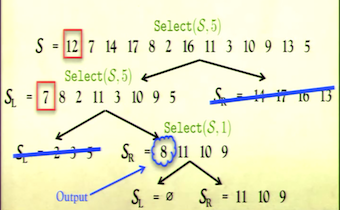
\includegraphics{lecture51}
\\
\item How many comparisons $T$(n) does this recursive selection algorithm make?
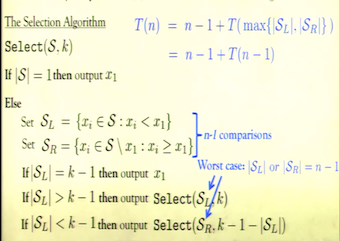
\includegraphics{lecture52}
\item So in the \textbf{worst case} we have is: \\
\\
{\large
$T$(n) = (n - 1) + $T$(n - 1)\\
\hspace*{9mm} = (n - 1) + (n - 2) + $T$(n - 2)\\
\hspace*{10mm} $\cdot$\\
\hspace*{10mm} $\cdot$\\
\hspace*{10mm} $\cdot$\\
\hspace*{9mm} = (n - 1) + (n - 2) + (n - 3) + $\cdot$ $\cdot$ $\cdot$ + 2 + 1\\
\hspace*{9mm} = {\Large$\frac{1}{2}$}n(n - 1)\\
\hspace*{9mm} = $\Omega$($n^2$)
}
\item This is terrible - sorting would have been faster!
\item How to fix it? Use Balanced Pivots!
 	\begin{itemize}
	\item The problem is the algorithm repeatedly \textbf{pivots} on the first number in the current list.
		\begin{itemize}
		\item But if we are unlucky this pivot could be very \textbf{unbalanced}. That is:\\
		{\large
		max$\{|S_L|, |S_R|\}$ $\approx$ n \\
		min$\{|S_L|, |S_R|\}$ $\approx$ 0
		}
		\end{itemize}
	\item What we would like is to select a pivot that is \textbf{balanced}. That is:\\
	{\large max$\{|S_L|, |S_R|\}$ $\approx$ $\frac{n}{2}$} \\
	{\large min$\{|S_L|, |S_R|\}$ $\approx$ $\frac{n}{2}$}
	\end{itemize}
\item Randomization
	\begin{itemize}
	\item The current algorithm is \textbf{deterministic} in the choice of the pivot.
	\item To fix the problem we consider a \textbf{randomized} implementation.
		\begin{itemize}
		\item Do not pivot deterministically on $x_1$.
		\item Instead choose the pivot at \underline{random} from $S$ = \{$x_1$, $x_2$, $\cdot$ $\cdot$ $\cdot$, $x_n$\}
		\end{itemize}
	\end{itemize}
{\large
\underline{Randomized Selection}\\
\\
\textbf{RandSelect}($S$, k)\\
\textbf{If} $|S|$ = 1 \textbf{then} output $x_1$\\
\textbf{Else}\\
\forceindent Pick a random pivot $x_{\tau} \in \{x_1, x_2, \cdot \cdot \cdot, x_n\}$\\
\forceindent Set $S_L$ = \{$x_i$ $\in$ $S$ : $x_i$ $<$ $x_{\tau}$\}\\
\forceindent Set $S_R$ = \{$x_i$ $\in$ $S$ $\setminus$ $x_{\tau}$ : $x_i$ $\geq$ $x_{\tau}$\}\\
\forceindent \textbf{If} $|S_L|$ = k - 1 \textbf{then} output $x_{\tau}$\\
\forceindent \textbf{If} $|S_L|$ $>$ k - 1 \textbf{then} output \textbf{RandSelect}($S_L$, k)\\
\forceindent \textbf{If} $|S_L|$ $<$ k - 1 \textbf{then} output \textbf{RandSelect}($S_R$, k - 1 - $|S_L|$)
}\\
\\
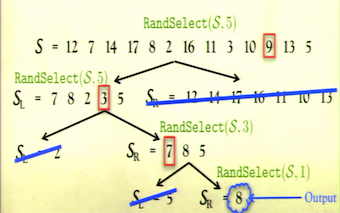
\includegraphics{lecture53}\\
\\
\item Good vs Bad Pivots
	\begin{itemize}
	\item Imagine all the numbers in the \textbf{sorted} order.\\
	\\
	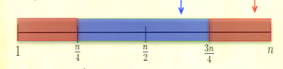
\includegraphics{lecture54}
	\item With probability $\frac{1}{2}$ the pivot $x_{\tau}$ lies between the 1st and 3rd quartiles.
		\begin{itemize}
		\item We say that such a pivot is \textcolor{blue}{good}.
		\item We say that such a pivot is \textcolor{red}{bad}.
		\end{itemize}
	\item \textbf{Key Observation}: If the pivot is good then \\
	\large{max$\{|S_L|, |S_R|\}$ $\leq$ $\frac{3}{4}$} $\cdot$ n\\
	\\
	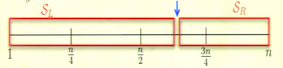
\includegraphics{lecture55}
	\end{itemize}
\item Expected Runtime
	\begin{itemize}
	\item In the worst case, the \textit{randomized algorithm} will pick the \underline{worst} pivot! The probability of its happening is very small.
	\item So, for randomized algorithms, we are always interested in the \textbf{expected runtime} $\bar{T}(n) = E(T(n))$, not the worst case run time.
	\item Using our observation, we then have that:\\
	\begin{center}
	\large{$\bar{T}(n) \leq \frac{1}{2} \cdot \bar{T}(\frac{3n}{4}) + \frac{1}{2} \cdot \bar{T}(n) + O(n)$}\\
	\end{center}
	Note: 
	\begin{enumerate}
	\item The first term: the probability of $\frac{1}{2}$ comes from I make a good pivot. If I make a good pivot, I know both of my subsets will have at most the size of  $\frac{3n}{4}$.
	\item The second term: If I get a bad pivot, the size of the next problem might be (n - 1), which is $\bar{T}(n)$ in the worst case.
	\end{enumerate}
	\hspace*{11mm}  {\large $\bar{T}(n) \leq \frac{1}{2} \cdot \bar{T}(\frac{3n}{4}) + \frac{1}{2} \cdot \bar{T}(n) + O(n)$}\\
	\\
	$\Rightarrow$ {\large $\frac{1}{2} \cdot \bar{T}(n) \leq \frac{1}{2} \cdot \bar{T}(\frac{3n}{4}) + O(n)$}\\
	\\
	$\Rightarrow$ \hspace*{5mm} {\large $\bar{T}(n) \leq \bar{T}(\frac{3n}{4}) + O(n)$}\\
	\item Apply the Master Theorem
		\begin{itemize}
		\item a = 1, b = $\frac{4}{3}$, and d = 1
		\item This is Case 1 of the Master Theorem.
		\item Runtime = $O(n^d)$ = $O(n)$
		\end{itemize}
	\end{itemize}
\end{itemize}

\section{Deterministic Selection}
\renewcommand{\labelitemii}{$\circ$}
\renewcommand{\labelitemiii}{$\cdot$}
\renewcommand{\labelitemiii}{$\rightarrow$}
\begin{itemize}
\item So we have a \textbf{linear time} \underline{randomized} algorithm for the selection problem.
\item Is there a linear time \underline{deterministic} algorithm?
\item To do this, what we need is a deterministic method to find a \textbf{good pivot}.
\item The idea is to find "the median of the medians."
\item Divide {\large $S = \{x_1, x_2, \cdot \cdot \cdot, x_n\}$} into groups of cardinality five:\\
{\large
$G_1 = \{x_1, \cdot \cdot \cdot, x_5\}, G_2 = \{x_6, \cdot \cdot \cdot, x_{10}\}, \cdot \cdot \cdot, G_{\frac{n}{5} } = \{x_{n-4}, \cdot \cdot \cdot, x_{n}\}$
}
\item Now sort each group and let $z_i$ be the median of the froup $G_i$\\
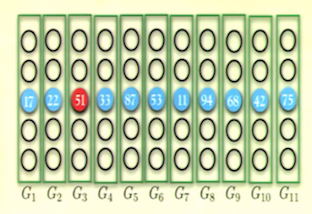
\includegraphics{lecture56}
\item Let \textcolor{red}{m} be the \textbf{median} of {\large $Z$ = \{$z_1$, $z_2$, $\cdot$ $\cdot$ $\cdot$, $z_{\frac{n}{5}}$\}}
\item As a thought experiment, \underline{reorder} the groups their median values:\\
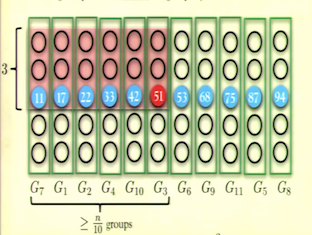
\includegraphics{lecture57}
\item The \textbf{median of the medians} is greater than at least {\large $\frac{3n}{10} - 1$ }numbers in $S$\\
\\
$\Rightarrow$     {\large $|S_R| = |\{x_i \in S \setminus m : x_i \geq m\}| \leq \frac{7}{10} \cdot n$}
\item There are at least {\large $\frac{3n}{10}  - 1$ } numbers in $S$ that are at least as big as m.\\
\\
$\Rightarrow$     {\large $|S_L| = |\{x_i \in S : x_i < m\}| \leq \frac{7}{10} \cdot n$}\\
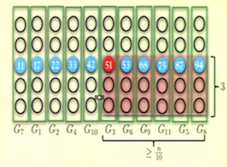
\includegraphics{lecture58}
\item Thus, using m as a \textbf{pivot} we have:\\
\\
$\Rightarrow$    {\large $max\{|S_L|, |S_R|\} \leq \frac{7}{10} \cdot n$}
\item Thus the median of the medians is a \textbf{good} pivot.
\item But how actually do we find the median of the medians?
	\begin{itemize}
	\item Using the same \textbf{deterministic recursive algorithm}!
	\end{itemize}
\end{itemize} 
;)
\\
\\
\\
\\
\\
\\
\\
\\
\\
\\
\\
\\
\\
\\
{\large \underline{Deterministic Selection}\\
\\
\textbf{DetSelect}($S$, k)\\
\textbf{If} $|S|$ = 1 \textbf{then} output $x_1$\\
\textbf{Else}\\
\forceindent Partition $S$ into [$\frac{n}{5}$] groups of 5.\\
\forceindent \textbf{For} $j = \{1,2, \cdot \cdot \cdot, \frac{n}{5}\}$\\
\forceindent \forceindent Let $z_j$ be the median of group $G_j$\\
\forceindent \textbf{Let} $Z = \{z_1,z_2, \cdot \cdot \cdot, z_{[\frac{n}{5}]}\}$\\
\forceindent Set m $\leftarrow$ \textbf{DetSelect}($Z$, [$\frac{n}{10}$])\\
\forceindent Set $S_L$ = \{$x_i$ $\in$ $S$ : $x_i$ $<$ m\}\\
\forceindent Set $S_R$ = \{$x_i$ $\in$ $S$ $\setminus$ \{m\} : $x_i$ $\geq$ m\}\\
\forceindent \textbf{If} $|S_L|$ = k - 1 \textbf{then} output m\\
\forceindent \textbf{If} $|S_L|$ $>$ k - 1 \textbf{then} output \textbf{DetSelect}($S_L$, k)\\
\forceindent \textbf{If} $|S_L|$ $<$ k - 1 \textbf{then} output \textbf{DetSelect}($S_R$, k - 1 - $|S_L|$)
}\\
\begin{itemize}
\item Thus, using m as a \textbf{pivot} we have:\\
\\
$\Rightarrow$    {\large $max\{|S_L|, |S_R|\} \leq \frac{7}{10} \cdot n$}
\item The recursive formula for the running time is then:\\
\\
$\Rightarrow$    {\large $T(n) \leq T(\frac{7n}{10}) + T(\frac{n}{5}) + O(n)$}\\
\\
Note: 
\begin{enumerate}
\item {\large $T(\frac{n}{5})$} term comes from finding the median of the medians.
\item {\large $T(\frac{7n}{10})$} comes from that pivoting on the median of the medians gives a significantly smaller  sub-problem.
\item {\large $O(n)$} comes from breaking in groups of size 5, finding the median of each group, and pivoting on the median of medians.
\end{enumerate}
\item But this does \textbf{not} fit with the Master Theorem!
	\begin{itemize}
	\item The problem is not broken into the same sized sub-problems. One is {\large $\frac{7n}{10}$}, the other is {\large $\frac{n}{5}$}.
	\end{itemize}
\item This does not matter as we understand the proof of the Master Theorem,\\
$\Rightarrow$   Apply the Recursion Tree Method!\\
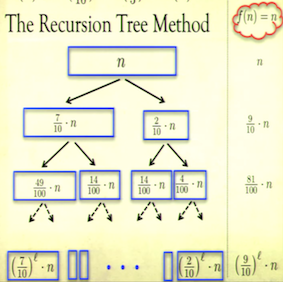
\includegraphics{lecture59}\\
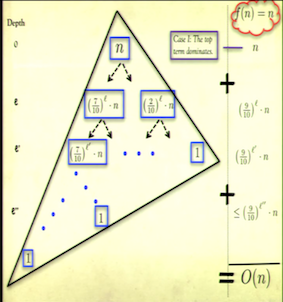
\includegraphics{lecture510}
\item Runtime: {\large $T(n) = O(n)$}
\item Thus, we have a deterministic \textbf{linear time} algorithm to solve the selection problem (and, specifically, to find the median).
	\begin{itemize}
	\item The reason why finding the selection problem is useful is that we try to find the median, but when we break it into two sub-problems, we are not finding the medians in the sub-problems since things would be shifted, and we might be finding the n over 10th problem. 
	\item This works a lot in induction. When you do induction proof, here we are using a stronger algorithm as our sub-routines, using kth selection problem, rather than median problem, which assumes that you have a stronger induction hypothesis. Often we use induction, it is hard to prove an easy result, since we can prove a general result, using induction.
	\end{itemize}
\end{itemize}



















\end{document}